\label{sec:dthreads-architecture}

\begin{figure}[!ht]
\fbox{
\subfigure{\lstinputlisting[frame=none,boxpos=t]{fig/mainthread.example.pseudocode}}
\hspace{10pt}
\subfigure{\lstinputlisting[numbers=none,frame=none,boxpos=t]{fig/thread1.example.pseudocode}}
\hspace{10pt}
\subfigure{\lstinputlisting[numbers=none,frame=none,boxpos=t]{fig/thread2.example.pseudocode}}
}
\caption{A simple multithreaded program with a race.\label{fig:sample}}
\end{figure}

Figure~\ref{fig:sample} shows a simple racey program that nondeterministically produces the outputs ``1,0,'' ``0,1'' and ``1,1.''  Because these threads access shared data without locks, modifications to shared state are immediately visible.  The order in which these modifications occur can change from run-to-run, resulting in nondeterministic output.  
Using \dthreads{}, this simple code will \emph{always} produce the output ``1,1," making it easy or the developer to reproduce and locate the data race.

\textbf{Threads as Processes:}
In \dthreads{}, threads are actually run as separate processes, an idea borrowed from Grace~\cite{grace}.  This means modifications by one thread are not visible to other threads until they are committed to global shared state.  Implementation is discussed in depth in Section~\ref{sec:threadsasprocs}.

%advantages (performance and isolation). Note that this is fast (point
%to Grace paper and BOP paper). Explain how it is based on clone, what
%flags are used, and why. Advantage: isolation. Costs are amortized.

\textbf{Deterministic Synchronization:}
To ensure deterministic execution, updates to shared state must be exposed at deterministic times, and in deterministic order.  \dthreads{} commits all modifications to shared state at thread creation, locks, condition variables, barriers, and thread exit.  Commits are ordered using a ``token'' that is passed from one thread to the next; a thread can only commit when it holds the token.  The token-passing protocol is described in Section~\ref{sec:token} and the implementation of synchronization primitives is described in Section~\ref{sec:synchronization}.

Rather than using retired instruction counts to demarcate commit
boundaries (as done by CoreDet and Kendo), \dthreads{} relies
exclusively on synchronization operations(different transactions). 
If there is no synchronization inside, each thread in \dthreads{} can run in
parallel. This approach dramatically increases performance for
computation-intensive workloads with little communication between
threads.

More importantly, these natural synchronization points
make \dthreads{} code more \emph{robust}: it is difficult for
programmers to know when a transaction ends if the boundary is the
number of instructions retired. That value can vary depending on the
underlying architecture and can also be input-dependent, meaning that
each different input may lead to completely different apparent thread
interleavings. By contrast, \dthreads{} guarantees that all code
between two synchronization points executes in isolation and all communications between
threads are executed according to one global order using the fence and token mechanism 
showed below.

\textbf{Shared Memory:} 
Because multithreaded programs frequently use updates to shared memory to communicate, \dthreads{} must implement a mechanism to expose one thread's updates to all other threads.  At the beginning of a transaction, all shared pages are protected, and can only be read by threads.  When a thread attempts to modify a shared page a local working copy is created, leaving the shared page unmodified.  At commit time, a ``twin'' copy of all modified pages is created.  Every page is compared to its twin (using a byte-wise diff) and modified bytes are copied back to the shared state.  Unlike transactional memory, conflicting changes do not result in rollbacks with \dthreads{}.  Further details are described in Section~\ref{sec:sharedmemory}.

\textbf{CCC: maybe move this toward the end of the section?}
For the code showed in Figure~\ref{fig:sample}, T1 and T2 are seeing \texttt{a=0} and \texttt{b=0} in the beginning. 
Then they check the value of \texttt{a} or \texttt{b} and updates correspondingly, since those updates won't be shared to 
another thread until the end of thread (in this case).
In the end of thread, each thread are committed in the order T1--T2, then \dthreads{} can print the results of ``1,1'' finally.

%\subsection{Threads as Processes}
% TTT: 
\subsection{Isolated Memory Access}
%\subsection{Threads as Processes}
\label{sec:threadsasprocs}
In order to achieve the deterministic memory access, 
\dthreads{} tries to isolate the memory access among different
threads in the beginning and commit those changes of different threads using a deterministic order.
%TTT end

To isolate the memory access among different threads, \dthreads{} are treating threads as processes.
In a multithreaded program running with pthreads, threads share all memory except for the stack.  Changes to memory are immediately visible to all other threads.  Threads share the same file descriptors, sockets, device handles, and windows.  Because \dthreads{} runs threads in separate processes, these shared resources must be explicitly managed by the runtime library.

\subsubsection{Thread Creation}
\dthreads{} replaces the \texttt{pthread\_create()} function.  Using the \texttt{clone} system call, \dthreads{} controls which resources are shared between processes.  The \texttt{CLONE\_FILES} flag (shown on line 3 of Figure~\ref{fig:threadcreation}), is used to create processes that share the same file descriptor table, but have distinct address spaces.

\subsubsection{Deterministic Thread Index}
\label{sec:threadindex}
POSIX does not guarantee deterministic process identifiers.  To avoid exposing this nondeterminism to threads running as processes, \dthreads{} uses an internal thread index and shims the \texttt{getpid()} function.  This internal thread index is managed using a single global variable that is incremented on thread creation.  This unique thread index is also used to manage per-thread heaps and as an offset into an array of thread entries.

%\subsubsection{Stack and Heap} 
% TTT: Change the title since we don't care about stack and add the mapping information, otherwise, it is not clear how we
% do that, it is very important to do so.
\subsubsection{Share Memory}
\label{sec:stackandheap}

In order to create the illusion of multi-threaded programs that
different threads are sharing the same address space, \dthreads{} uses
memory mapped files to share the globals and heap across different
processes. Note that \dthreads{} does not try to share the stack across
different processes (see Section~\ref{sec:discussion}).

\dthreads{} creates two different mappings for both the heap and the
globals.  One is a shared mapping, which is used to hold shared state.
The other is a private, copy-on-write (COW) per-process mapping that
each process works on directly.  Private mappings are linked to the
shared mapping through the one fixed-size memory mapped file.
Reads initially go directly to the shared mapping,
but after the first write operation,
both reads and writes are entirely private.
%TTT_end
Memory allocations are issued from the shared heap memory using a scalable per-thread heap organization loosely based on Hoard~\cite{BergerMcKinleyBlumofeWilson:ASPLOS2000} and built using HeapLayers~\cite{BergeZornMcKinley:2001}.  \dthreads{} divides the heap into a fixed number of sub-heaps (currently 16).  Each thread uses a hash of its thread index to find the appropriate sub-heap.

%\subsection{Shared Memory} 
% TTT: Change the title
\subsection{Deterministic Memory Commit}
\label{sec:sharedmem}

\begin{figure}
{\centering 
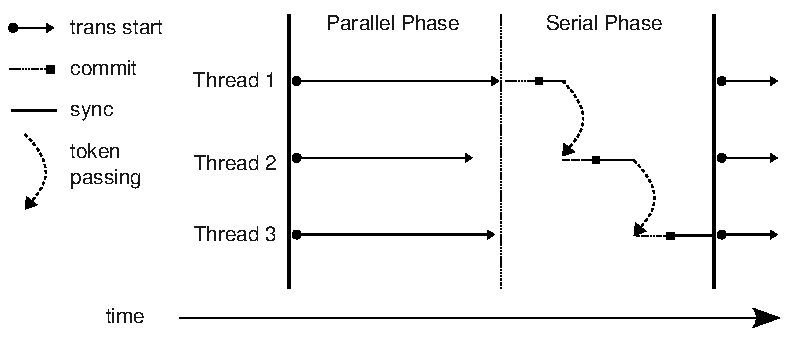
\includegraphics[width=3.25in]{fig/phase}
\caption{An overview of \dthreads{} phase. Program execution with \dthreads{} parallel and serial phases.\label{fig:phase}}
}
\end{figure}

Figure~\ref{fig:phase} illustrates the progression of parallel and serial phases. 
To guarantee determinism, \dthreads{} isolates memory accesses in parallel phase. Those memory accesses in
parallel phase can work on their private copies of different process safely, those updates won't be exposed to 
shared state in parallel phase.
When a synchronization point is reached, updates are exposed in deterministic order.  
This section describes the mechanism used to alternate between parallel and serial execution 
and guarantee deterministic commit order, and the details of commits to shared memory.

\subsubsection{Fence and Token}
% TTT: don't agree with "a global lock".
%\subsubsection{\dthreads{} Schedule}
\label{sec:schedule}

The boundary between the parallel and serial phase is the internal fence.  
It is not possible to implement the internal fence using the \texttt{pthreads} barrier 
because the number of threads required to proceed can change during execution and the \texttt{pthreads} barrier does not provide this functionality (details in Section~\ref{sec:synchronization}).

\label{sec:token}
\begin{figure}
\begin{lstlisting}
void waitFence(void) {
	lock();
	while(!isArrivalPhase()) { 
		CondWait();
	}

	waiting_threads++;
	if(waiting_threads < live_threads) {
		while(!isDeparturePhase()) {
			CondWait();
		}
	} else {
		setDeparturePhase();
		CondBroadcast();
	}

	waiting_threads--;
	if (waiting_threads == 0) {
		setArrivalPhase();
		CondBroadcast();
	}
	unlock();
}
\end{lstlisting}
\caption{Pseudocode for the internal fence.\label{fig:internalFence}}
\end{figure}

Figure~\ref{fig:internalFence} shows pseudocode for the internal fence.  Threads must wait at the fence 
until all threads from the previous 
% TTT
%parallel have departed (lines 3-5).  
%Once the fence has emptied of threads,
% Once all previous 
fence have deptarted. Those waiting threads should block until the departure phase (lines 8-11). 
% TTT_end
If the thread is the last to enter the fence, it sets the departure phase and wakes the waiting threads (lines 12-15).  
As threads leave the fence, they decrement the waiting thread count.  The last thread to leave sets the fence to the arrival phase and wakes any waiting threads (lines 17-21).

\textbf{CCC: Not edited}

\begin{figure}
\begin{lstlisting}
void waitToken() {
  waitFence();
  while(isNotMyToken()) { yield(); }
}
void putToken() {
    passTokenToNextOfTokenQueue();
}
\end{lstlisting}
\caption{Pseudocode for waitToken and putToken. waitToken() first waits at the fence (line 2) and then waits for
the token to be set to current thread (line 3).  putToken() simply
passes the token to the next thread entry in the token queue.
\label{fig:token}}
\end{figure}

Another important mechanism of \dthreads{} is the token implementation. 
In order to guarantee determinism, each thread must wait for token
before it can communicate with other threads. 
The token is one shared pointer actually, pointing to next runnable thread entry.
Since the token is unique in the whole system, it guarantees a global order for
all operations in serial phase. 

We introduce two subroutines to manage tokens. \texttt{waitToken()}
waits at the internal fence and then waits to acquire the global token
in order to enter serial mode. \texttt{putToken()} passes the token to
the next waiting thread.

To achieve determinism (see Figure~\ref{fig:phase}), those threads from parallel phase 
should wait at the internal fence before they can entering into the serial phase (actually calling
\texttt{waitToken}).
Note that it is important to wait at fence even for one thread which doomed to win the token next,
since their commits can affect other threads' behavior if no fence.
In serial phase, each thread can do those commits for parallel phase and actual synchronizations
before they passed the token to next thread. 
In the end of serial phase, we still needs to wait at fence in order to entering into next run for the same reason.


\textbf{CCC: Edited}

\subsubsection{Commit Protocol}
\begin{figure}
{\centering
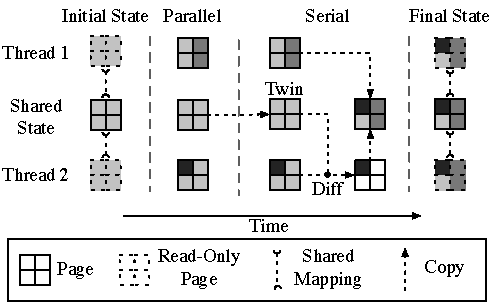
\includegraphics[width=3.25in]{fig/architecture-diagram}
\caption{An overview of \dthreads{} execution.\label{fig:architecture}}
}
\end{figure}

Figure~\ref{fig:architecture} shows the steps taken by \dthreads{} to capture modifications to shared state and expose them in a deterministic order.  At the beginning of the parallel phase, threads have a read-only mapping for all shared pages.  If a thread writes to a shared page during the parallel phase, this write is trapped and re-issued on a private copy of the shared page.  Reads go directly to shared memory and are not trapped.  In the serial phase, threads commit their updates one at a time.  The first thread to commit to a page can directly copy its private copy to the shared state, but subsequent commits must copy only the modified bytes.  This is done by diffing with the twin page, an unmodified copy of the shared page from the beginning of the serial phase.  At the end of the serial phase, private copies are released and these addresses are restored to read-only mappings of the shared memory.

\textbf{CCC: It looks like pages are write-protected in atomicBegin AND atomicEnd.  This seems redundant.}

\begin{figure}[!ht]
\begin{lstlisting}
void atomicBegin() {
	foreach(page in modifiedPages) {
		page.writeProtect();
		page.privateCopy.free();
	}
	// CCC: what does this next line do?
	cleanupDirtyPagelist(); 
}
\end{lstlisting}
\caption{Pseudocode for \texttt{atomicBegin}.\label{fig:atomicbegin}}
\end{figure}

\label{sec:atomicbegin}

Figure~\ref{fig:atomicbegin} shows pseudocode for the \texttt{atomicBegin()} function.   First, all previously-written pages are write-protected (line 3).  The old working copies of these pages are then discarded, and mappings are updated to reference the shared state (line 4).

\begin{figure}[!ht]
\begin{lstlisting}
void atomicEnd(bool doCleanup) {
	foreach(page in modifiedPages) {
		if(page.writers > 1 && !page.hasTwin()) {
			page.createTwin();
		}

		if(page.version == page.localCopy.version) {
			page.copyCommit();
		} else {
			page.diffCommit();
			// CCC: Why isn't this outside the 'if'?
			if(doCleanup) {
				page.writeProtect();
				page.privateCopy.free();
			}
		}

		page.writers = page.writers - 1;
		if(page.writers == 0 && page.hasTwin()) { 
			page.twin.free();
		}
		page.version = page.version + 1;
	}
}
\end{lstlisting}
\caption{Pseudocode for \texttt{atomicEnd}.\label{fig:atomicend}}
\end{figure}

Figure~\ref{fig:atomicend} shows the pseudocode for the \texttt{atomicend()} function.  \texttt{atomicEnd()} commits all changes from the current transaction to the shared page.  For each modified page with more than one writer, \dthreads{} ensures that a twin page is created (lines 3-5).  If the version number of the private copy matches the shared page, then this is the first thread to commit.  In this case, the entire private copy can be copied to the shared state (lines 7 and 8).  If the version numbers do not match, then another thread has already committed changes to the page and a diff-based commit must be used (lines 9-10).  If the \texttt{doCleanup} flag is set, the page is write-protected and the private copy is freed (lines 12-15).  The number of writers to the page is decremented (line 18), and if there are no writers left to commit, the twin page is freed (lines 19-21).  Finally, the shared page's version number is incremented (line 22).

\textbf{CCC: Not Edited}

\subsection{Deterministic Synchronization}
\label{sec:synchronization}

Comparing to Grace, \dthreads{} supports one complete synchronization
mechanism.  Grace turns lock operations to no-ops to eliminate
deadlocks and does not support conditional variables or barriers.  The
only supported synchronization by Grace is thread exit; Grace enforces
a sequential semantics in thread exit.

\dthreads{} supports the full range of synchronizations in the
pthreads API, including locks, conditional variables, barriers and
different kinds of thread exit.

\subsubsection{Locks}

\dthreads{} does not differentiate between specific locks by using the same global token, 
which can possibly compromise the efficiency of program. But we argue
that it is necessary to do so in order to get the complete
deterministic view of memory in the share-memory model.
Multiple locks are treated as one lock, and serial mode ends
when all locks have been unlocked. 
% EDB: We need to acquire a token before we can execute any
% synchronization operation. We only release the token once our lock
% count is 0 (for instance, lock(A); lock(B); unlock(B); unlock(A);
% we release the token only after unlock(A).


% (more reasons ******).

% critical sections are normally short, so...

\begin{figure}
\begin{lstlisting}
void mutex_lock (pthread_mutex_t * mutex) {
  if(_locks == 0) {
    waitToken();
    atomicEnd(true);
  }
  _locks++;
}
\end{lstlisting}
\begin{lstlisting}
void mutex_unlock(pthread_mutex_t * mutex) {
  _locks--;
  // Release the token when no locks are held.
  if(_locks == 0) {
    atomicEnd(false);
    putToken();
    atomicBegin();
    waitFence();
  }
}
\end{lstlisting}
\caption{Pseudocode for lock and unlock($\S$~\ref{sec:lock}).
\label{fig:lock}}
\end{figure}

\label{sec:lock}
Figure~\ref{fig:lock} presents pseudocode for \texttt{lock and unlock}.
First, it will check whether current threads has already held the token(line 2). 
If not, then current thread should wait the token in order to enter into 
the serial phase(line 3). The first thing in the serial phase is to
commit those changes of current transaction to the shared mapping and 
do some basic cleanup (line 4) (see ~\ref{sec:atomicBegic}).
In unlock(), we decrement the count for lock (line 2) and don't do anything if
lock is no equal to 0, which makes multiple locks behaving as a huge lock, potentially 
avoiding any possible deadlock problems.
If lock's count is equal to 0, we commit all memory modifications (line 5) and release
the token to next thread in the token queue (line 6). Then it can do self cleanup by calling
\texttt{atomicBegin}. After that, it simply wait at the fence in order to enter into the next
round's parallel phase (line 8).

\subsubsection{Condition Variables}

Guaranteeing determinism for condition variables is more complex than
for other synchronization operations. In this case, \dthreads{} cannot
rely on operating system support, since threads waiting on the same
condition variable can be awakened in any order. In addition, naively
imposing a global order could easily lead to deadlocks.

\label{sec:condwait}
Different with the busy wait mechanism that CoreDet used, 
\dthreads{} tries to reduce the performance cost
introduced by busy wait mechanism. Since we have no idea when those
waiting threads will be awakened, we don't want those threads to be
checked frequently since this can cause expensive process
switches. Also, we don't want those waiting threads to thwart the the
token passing of non-waiting threads.
In \dthreads{}, waiting threads are extracted from the normal run
queue and inserted into the corresponding queue of condition
variable so that the token will not be passed to these waiting
threads.

By inserting threads into corresponding queue of condition
variables, which can help those signal and broadcast function to find
out which thread should be waken up firstly and to avoid the
un-determinism brought by operating system. We enforce the
first-in-first-out rule for all waiting threads.

Since those threads calling \texttt{cond\_wait} should get the token in order
to ensure the determinism, they have to release the token to next
thread in the active list. After finishing these work, then those
threads can actuall waiting on the real process-shared conditional
variable.

After one thread is awakened, the thread should try to get token at
first in order to proceed since the thread being awakened is 
still inside the critical section (under lock protection)
and the token is required to guarantee determinism under the critical region. 

\dthreads{} uses the busy wait mechanism to get the global token. 
It is noted that this new awakened thread don't need to call waitToken() to get
token since waitToken() should wait for all alivethreads to reach the fence at first. 
Now the waking thread has already passed the fence, calling waitToken() can potentially
put this new awakened thread to the next run of serial phase, which not only hurts
the performance but also introduce some possible deadlock.

\begin{figure}
\begin{lstlisting}
void cond_wait (pthread_cond_t * cond) {
  waitToken();
  atomicEnd(false);
  removeFromTokenQueue();
  insertToTailOfCondqueue();
  decreaseInternalFence();
  putToken();
  // Only proceed if I am ready to run.
  while (!isReadyToGo()) { real_condwait(); }
  while (isNotMyToken()) { yield(); } 
  atomicBegin();
  // Token can be released in unlock. 
}
\end{lstlisting}
\caption{Pseudocode for \texttt{cond\_wait} ($\S$~\ref{sec:condwait}). 
\label{fig:condwait}}
\end{figure}

Figure~\ref{fig:condwait} presents pseudocode
for \texttt{cond\_wait}.  When a thread executes \texttt{cond\_wait},
it first awaits the token (line 2) before it can proceed.  It then
commits local modifications, removes itself from the token queue, and
places itself at the tail of conditional variable's queue (lines
3--5). It then decreases the internal fence thread count (line 6) and passes
the token to the next entry on the token queue (line 7). When a thread
is awakened by a signal, it checks whether the current thread is in
fact ready to run (line 9), since multiple threads can be awakened
by \texttt{cond\_signal} but only the first thread can run.  Finally,
it waits for the token to enter into the serial phase (line 12). 

\label{sec:condsignal}

\begin{figure}
\begin{lstlisting}
void cond_signal() {
  if(!isHoldingToken())
    waitToken();
  atomicEnd(false);
  if(noWaiters()) return;
  lock();
  thread = getFirstThreadOfCondQueue();
  insertToHeadOfTokenQueue();
  setThreadReadyToGo();
  incrementInternalFence();
  unlock();
  atomicBegin();
}
\end{lstlisting}
\caption{Pseudocode for \texttt{cond\_signal} ($\S$~\ref{sec:condsignal}). 
\label{fig:condsignal}}
\end{figure}

In \texttt{pthreads}, the only difference between \texttt{cond\_signal}
and cond\_broadcast is that \texttt{cond\_signal} only wakes up the
first thread, while cond\_broadcast wakes up all threads in the
queue. To guarantee determinism for \texttt{cond\_signal}, \dthreads{}
broadcasts the signal to all threads blocked on the condition
variable, but only the status of first thead in the queue can be set
to runnable, so other threads will have to wait on the condition
variable again (see~\ref{fig:condwait}).
These functions remove the corresponding threads from the queue
of condition variable and insert them to the header of active list,
thus those threads can get token next.  Note that it is very important
to do so both to avoid deadlock and to improve performance. By placing
awakened theads on the next runnable position rather than on the tail
of the run queue, \dthreads{} avoids possible deadlocks. 
Thus, these awakened threads can run immediately (see line 10 of Figure~\ref{fig:condwait}) 
after getting the token, which improves performance. Finally, the
signalling thread releases the token to awakened threads.

Figure~\ref{fig:condsignal} presents the pseudocode
for \texttt{cond\_signal}. Before proceeding, the caller waits for
the token if it is not holding it already, and commits any local
modifications (lines 2--4).  If there are no waiters on the
conditional variable, it returns immediately. Otherwise, \dthreads{}
removes the first thread from the condvar's queue and places it at the
head of the token queue (lines 7--8). Finally, it makes this thread
runnable and increase the internal fence's thread count (line 9--10).

\subsubsection{Barriers}

\label{sec:barrierwait}

\begin{figure}
\begin{lstlisting}
void barrier_wait() {
  waitToken(); atomicEnd(false);
 
  lock();
  if(isLastThreadEnterBarrier()) {
	moveWholelistBacktoTokenqueue();
	increaseInternalFence(waitersNumb);
	passTokenToFirstOfBarrQueue();
  } 
  else {
    removeFromTokenqueue();
	insertTailOfBarrQueue();
	putToken();
  }
  unlock();

  atomicBegin();
  realBarrierWait();  
}
\end{lstlisting}
\caption{Pseudocode for barrier\_wait ($\S$~\ref{sec:barrierwait}).
\label{fig:barrierwait}}
\end{figure}

As with condition variables, \dthreads{} must ensure that threads
waiting on a barrier do not disrupt the token passing of running
threads. \dthreads{} removes threads entering into the barrier from
the run queue and places them on the corresponding barrier queue.

To avoid blocking on the barrier, the last thread entering into
the barrier moves all threads to the runnable queue and increases
the fence's thread count.

To improve parallelization, atomicBegin() is called to write-protect 
all dirty pages and release private copies before they actually wait on 
the real process-shared barrier. Thus, the work of atomicBegin() runs in parallel
with other threads. 

Figure~\ref{fig:barrierwait} presents pseudocode
for \texttt{barrier\_wait}. The calling thread first waits for the
token to commit any local modifications in order to ensure
deterministic commit (lines 2 and 3). If the current thread is the
last to enter the barrier, then \dthreads{} moves the entire list of
threads on the barrier queue to the token queue (line 7), increases
the fence's thread count (line 8), and passes the token to the first thread in the
barrier queue (line 9).  Otherwise, \dthreads{} removes the current
thread from the token queue (line 12), places it on the barrier queue
(line 13), and releases token (line 14). Finally, the thread waits on
the actual barrier (line 19).

\subsubsection{Thread Creation and Exit}

\label{sec:threadcreation}

\begin{figure}
\begin{lstlisting}
void thread_create () {
  waitToken();
  clone(CLONE_FS| CLONE_FILES | CLONE_CHILD);
  if(isChild) {
    getGlobalThreadIndex();
	insertToTokenQueue();
	notifyChildRegistered();
	// Await notification until parent reaches 
    // next sync point after spawning.
	waitParentBroadcast();	
  }
  else if (isParent) {
	waitChildRegistered();
  }
}
\end{lstlisting}
\begin{lstlisting}
void thread_exit() {
  waitToken();
  atomicEnd(false);
  removeFromTokenQueue();
  decreaseInternalFence();
  putToken();
  exitThread(); 
}
\end{lstlisting}
\caption{Pseudocode for thread creation and exit ($\S$~\ref{sec:threadcreation}).
\label{fig:threadcreation}
}
\end{figure}

\textbf{CCC: Edited}

To guarantee determinism, thread creation and exit must be performed in the serial phase.  Newly created threads are immediately added to the token queue.  Creating a thread does not immediately release the token; this allows a single thread to quickly create multiple child threads without waiting for a new serial phase for each.

Figure~\ref{fig:threadcreation} shows pseudocode for thread creation. The caller first waits for the token before proceeding (line 2).  It then creates a new process with shared file descriptors but a distinct address space using the \texttt{clone} system call (line 3).  The newly created child obtains the global thread index (line 5), places itself in the token queue (line 6), and notifies the parent that child has registered itself in the active list (line 7). The child thread then waits for the parent to reach a synchronization point.

When \texttt{thread\_exit()} is called, the caller first waits for the token and then commits any local modifications (line 3). It then removes itself from the token queue (line 4) and decreases the number of threads required to proceed to the next phase (line 5). Finally, the thread passes its token to the next thread in the token queue (line 6) and exits (line 7).

\textbf{CCC: Not Edited}

\subsubsection{Thread Cancellation}

\dthreads{} provides the following mechanism to support
deterministic thread cancellation. First, thread cancellation can only
happen in the serial mode withholding the token, which guarantees that
only current thread trying to issue cancellation request is
running. Other threads are either waiting on condition variables or
barriers. Second, thread entry should have enough information about
their status, which can be recorded. If one thread being cancelled are
waiting on condition variable or barrier, it should be removed from
corresponding queue in order to guarantee the correctness.

\subsection{Racey Example}
% return to racey example from the top of the section, walk through an execution with dthreads

\subsection{Optimizations}
\dthreads{} does a lot of optimizations to improve the performance.

\subsubsection{Optimization for One Thread}
When only one thread is running, \dthreads{} does not provide memory protection 
and treats all synchronization operations as no-ops.

\subsubsection{Lazy Twin Creation}
Twin pages are only created when a page has multiple writers during the same transaction.  
During the commit phase, the single writer can directly copy its working copy to the shared state 
without performing a diff.  This reduces the overhead in the common case, 
where a single thread is the exclusive writer of a page.

\subsubsection{Commit Optimization}
If one thread is the only writer on one page or it is the first thread to commit a page,
they can directly copy its working copy to shared state.
We are relying on one global page version number to check that in implementation. 
In the page handler, each thread can save one version number for every dirty page. 
In the commit process, \dthreads{} could compare this local version number with global version
number to check whether this is the first writer (see Figure~\ref{fig:atomicBegin} for pseudo code).
Any other threads that have written to this page must perform a diff against the twin page.

Another optimization is to do parallization as much as possible. 
\texttt{atomicBegin} only does some laundry jobs, releasing those private page frames or resetting pages to read-only mode.
We are trying to make this to parallize with other works since it only affect one threads' behavior. 
For example, \texttt{atomicEnd} in lock operations (see Figure~\ref{fig:lock} 
not only commits, but also launders pages if
necessary. Clearly, it is safe to cleanup all dirty pages but that
brings the performance problem since it is finished in serial phase.
By using the \texttt{atomicEnd(true)}, only those pages modified by
earlier threads should be cleaned up in order to give one complete
image of one page which later transactions may refer to.
